\documentclass{article}
    \usepackage{url}
    \usepackage[margin=1.0in]{geometry}
    \usepackage{cite}    
    \usepackage{amssymb}
    \usepackage{enumerate}
    \usepackage{enumitem}
    \usepackage{graphicx}
    \usepackage{xcolor}
    \usepackage{pdfpages}
    \usepackage{hyperref}
    \usepackage{listings}
    \usepackage{fancybox}
    \usepackage{lstautogobble}
    \usepackage{titling}
    \usepackage{pdflscape}
    \usepackage{afterpage}
    \usepackage[nottoc,notlot,notlof]{tocbibind}
    \renewcommand\maketitlehooka{\null\mbox{}\vfill}
    \renewcommand\maketitlehookd{\vfill\null}

    \newcommand\arduinobackgroundimage{
        \put(-5,0){
        \parbox[b][\paperheight]{\paperwidth}{
        \vfill
        \centering
        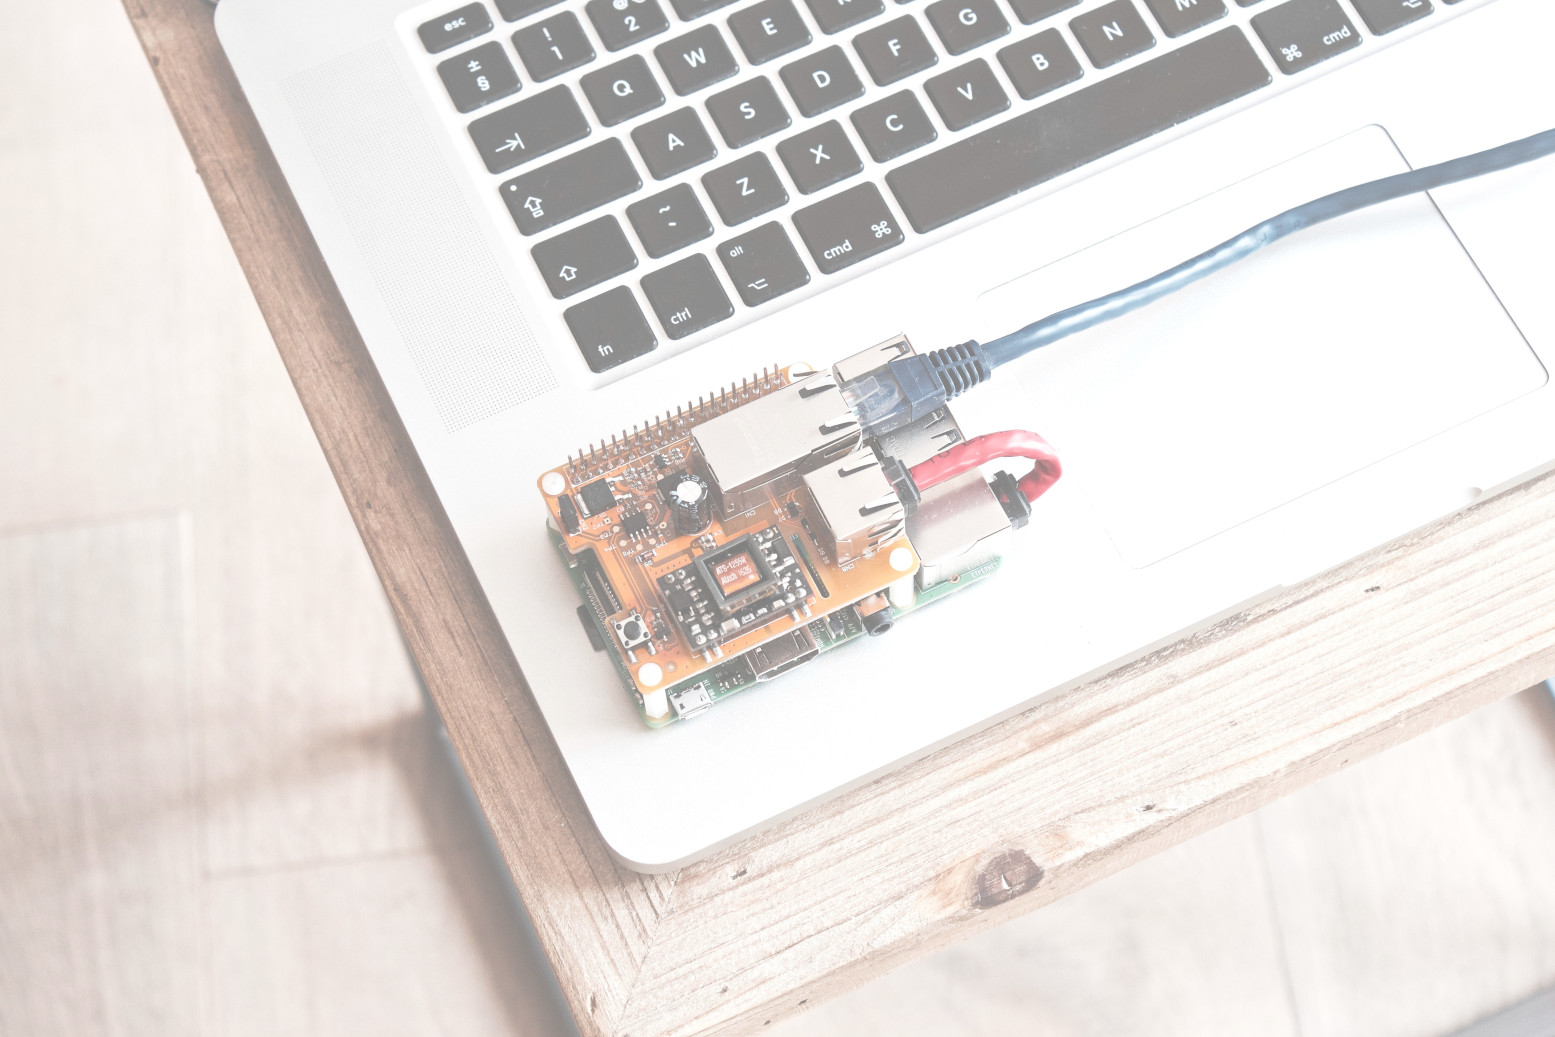
\includegraphics[height=\paperheight]{Images/Arduino.jpg}
        \vfill
    }}}

    \newcommand\usbdocumentbackgroundimage{
        \put(-5,0){
        \parbox[b][\paperheight]{\paperwidth+5px}{
        \vfill
        \centering
        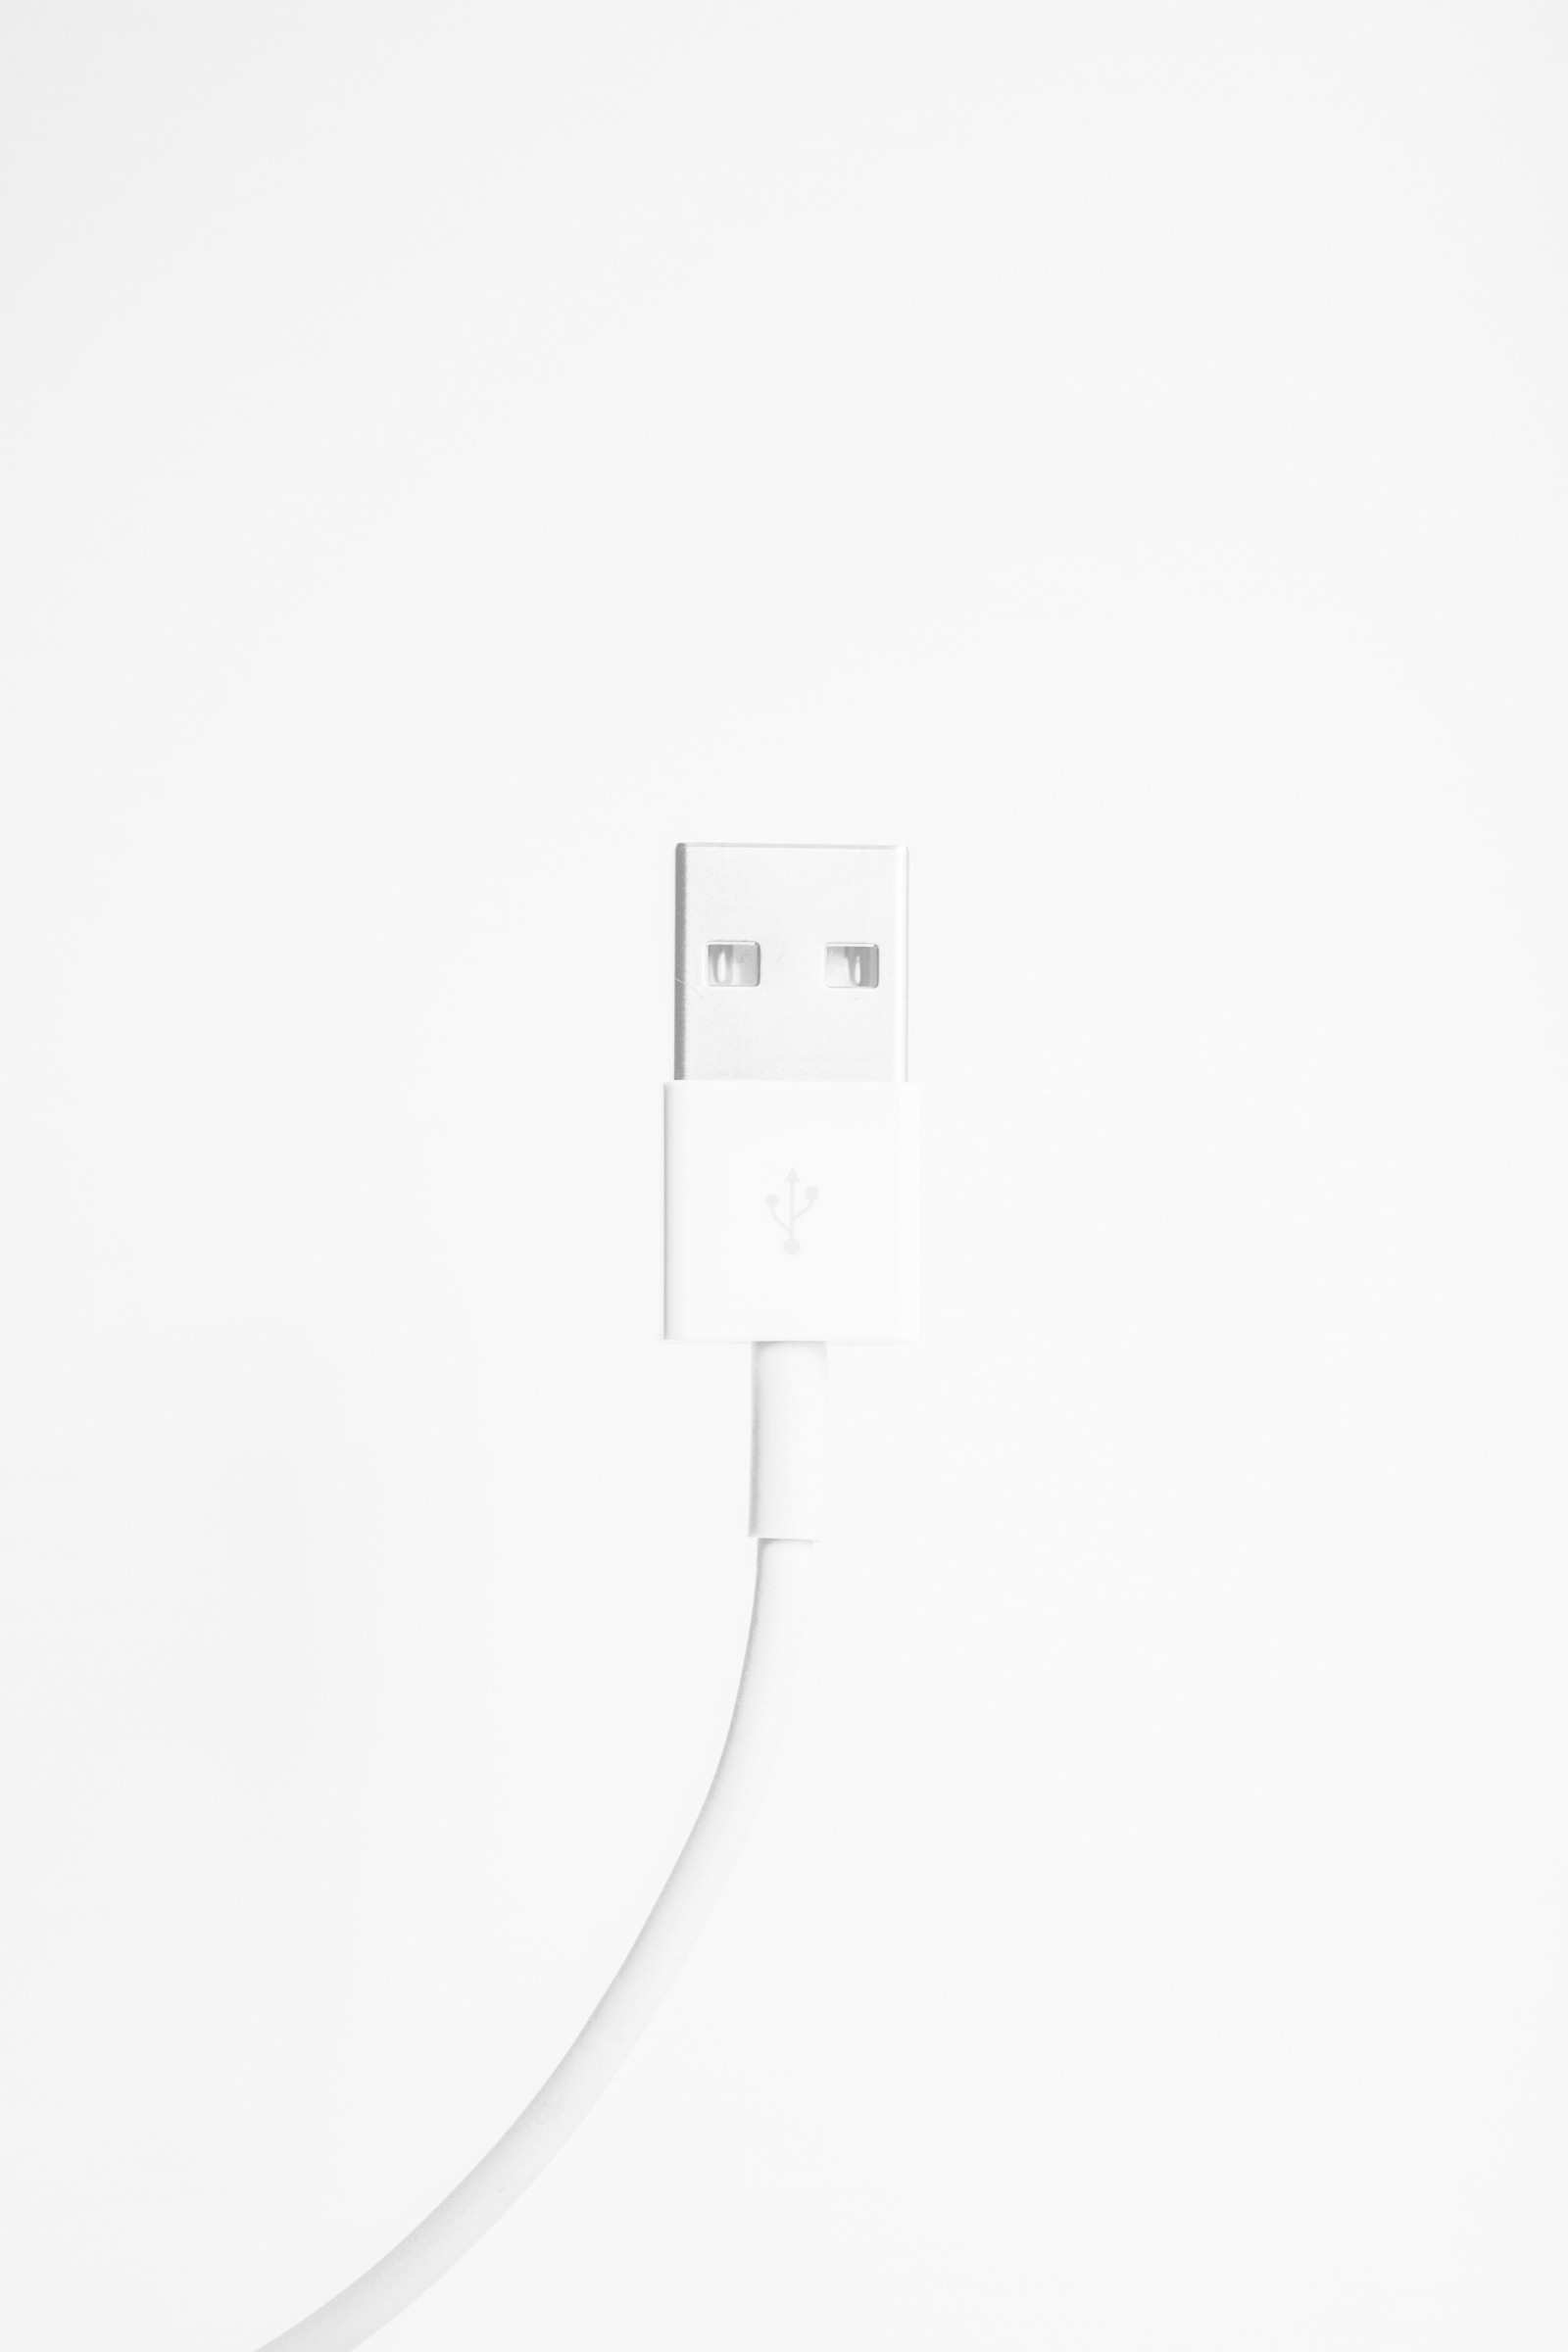
\includegraphics[width=\paperwidth]{Images/USB.jpg}
        \vfill
    }}}

    \newcommand\dronebackgroundimage{
        \put(-5,0){
        \parbox[b][\paperheight]{\paperwidth+5px}{
        \vfill
        \centering
        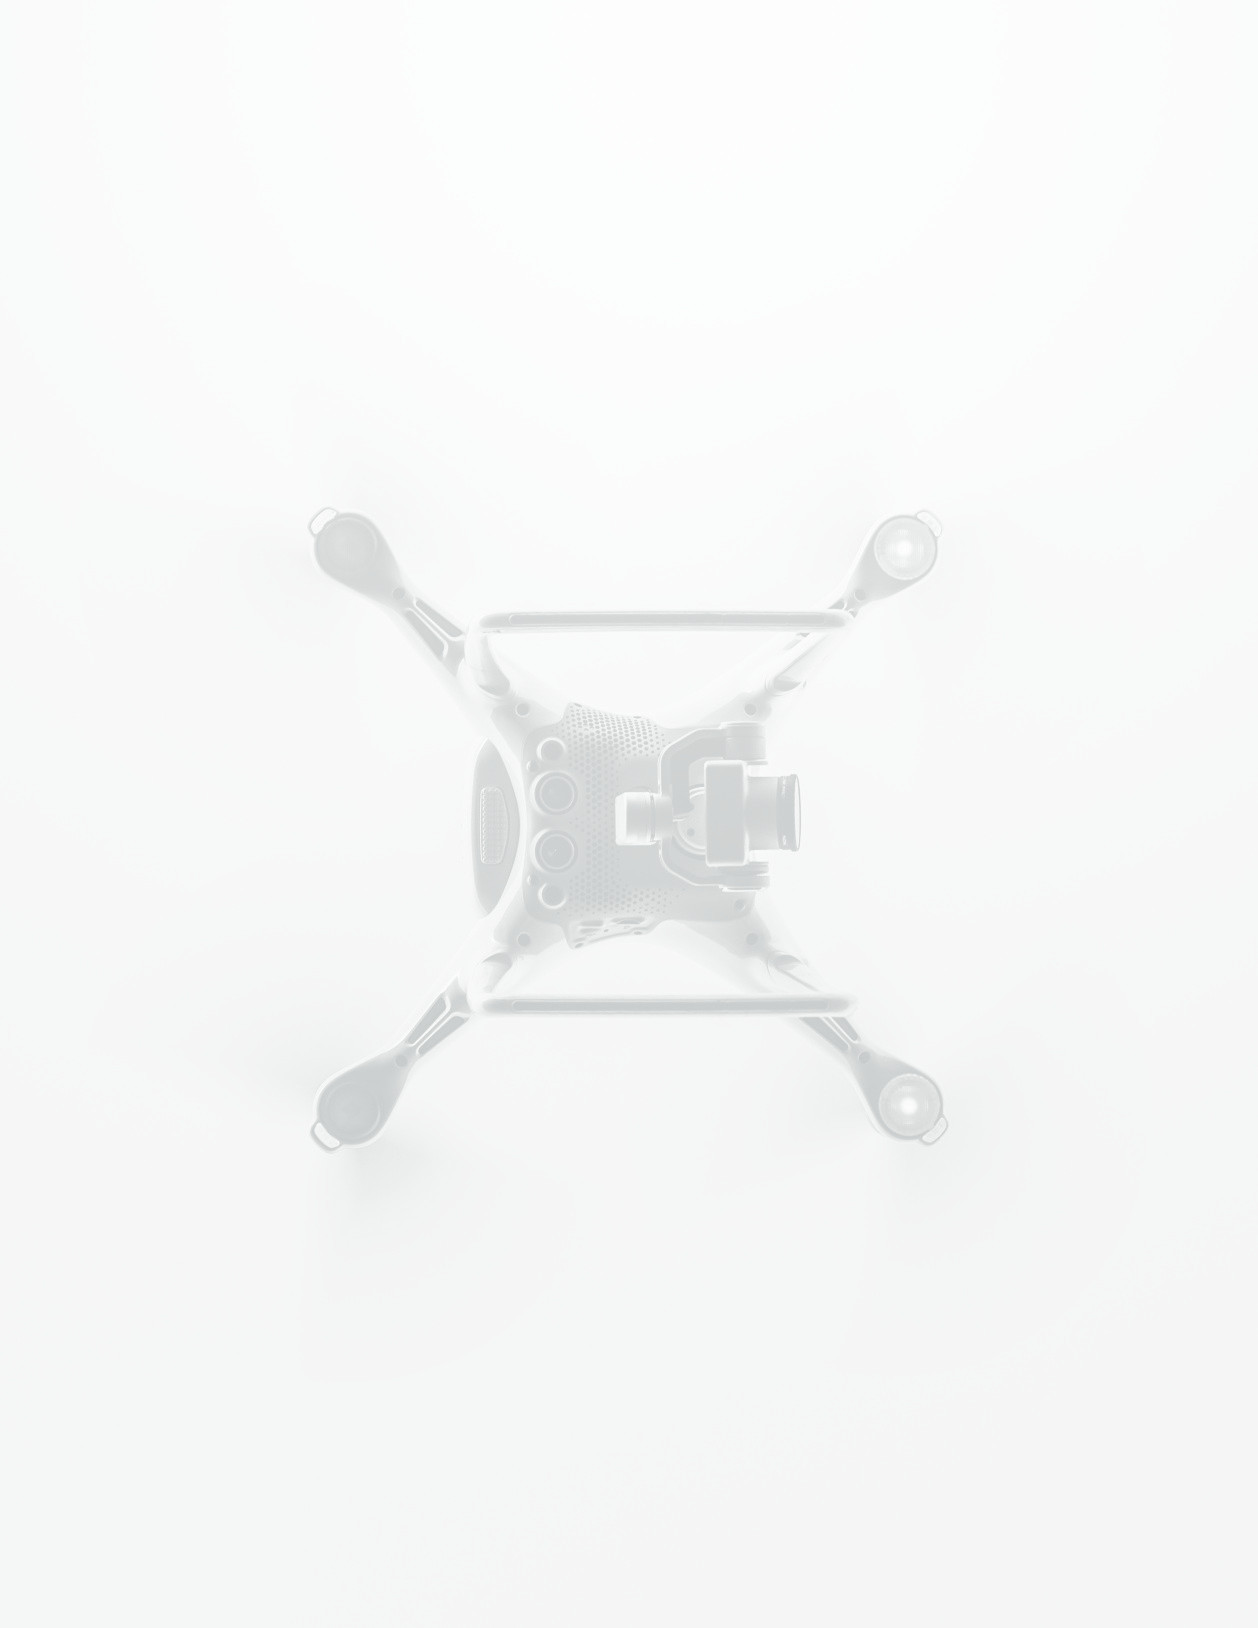
\includegraphics[width=\paperwidth]{Images/Drone.jpg}
        \vfill
    }}}

    \newcommand\whitebackgroundimage{
        \put(-5,0){
        \parbox[b][\paperheight]{\paperwidth}{
        \vfill
        \centering
        
\includegraphics[height=\paperheight]{Images/Gradient.jpg}
        \vfill
    }}}

    \newcommand\boardbackgroundimage{
        \put(-5,0){
        \parbox[b][\paperheight]{\paperwidth}{
        \vfill
        \centering
        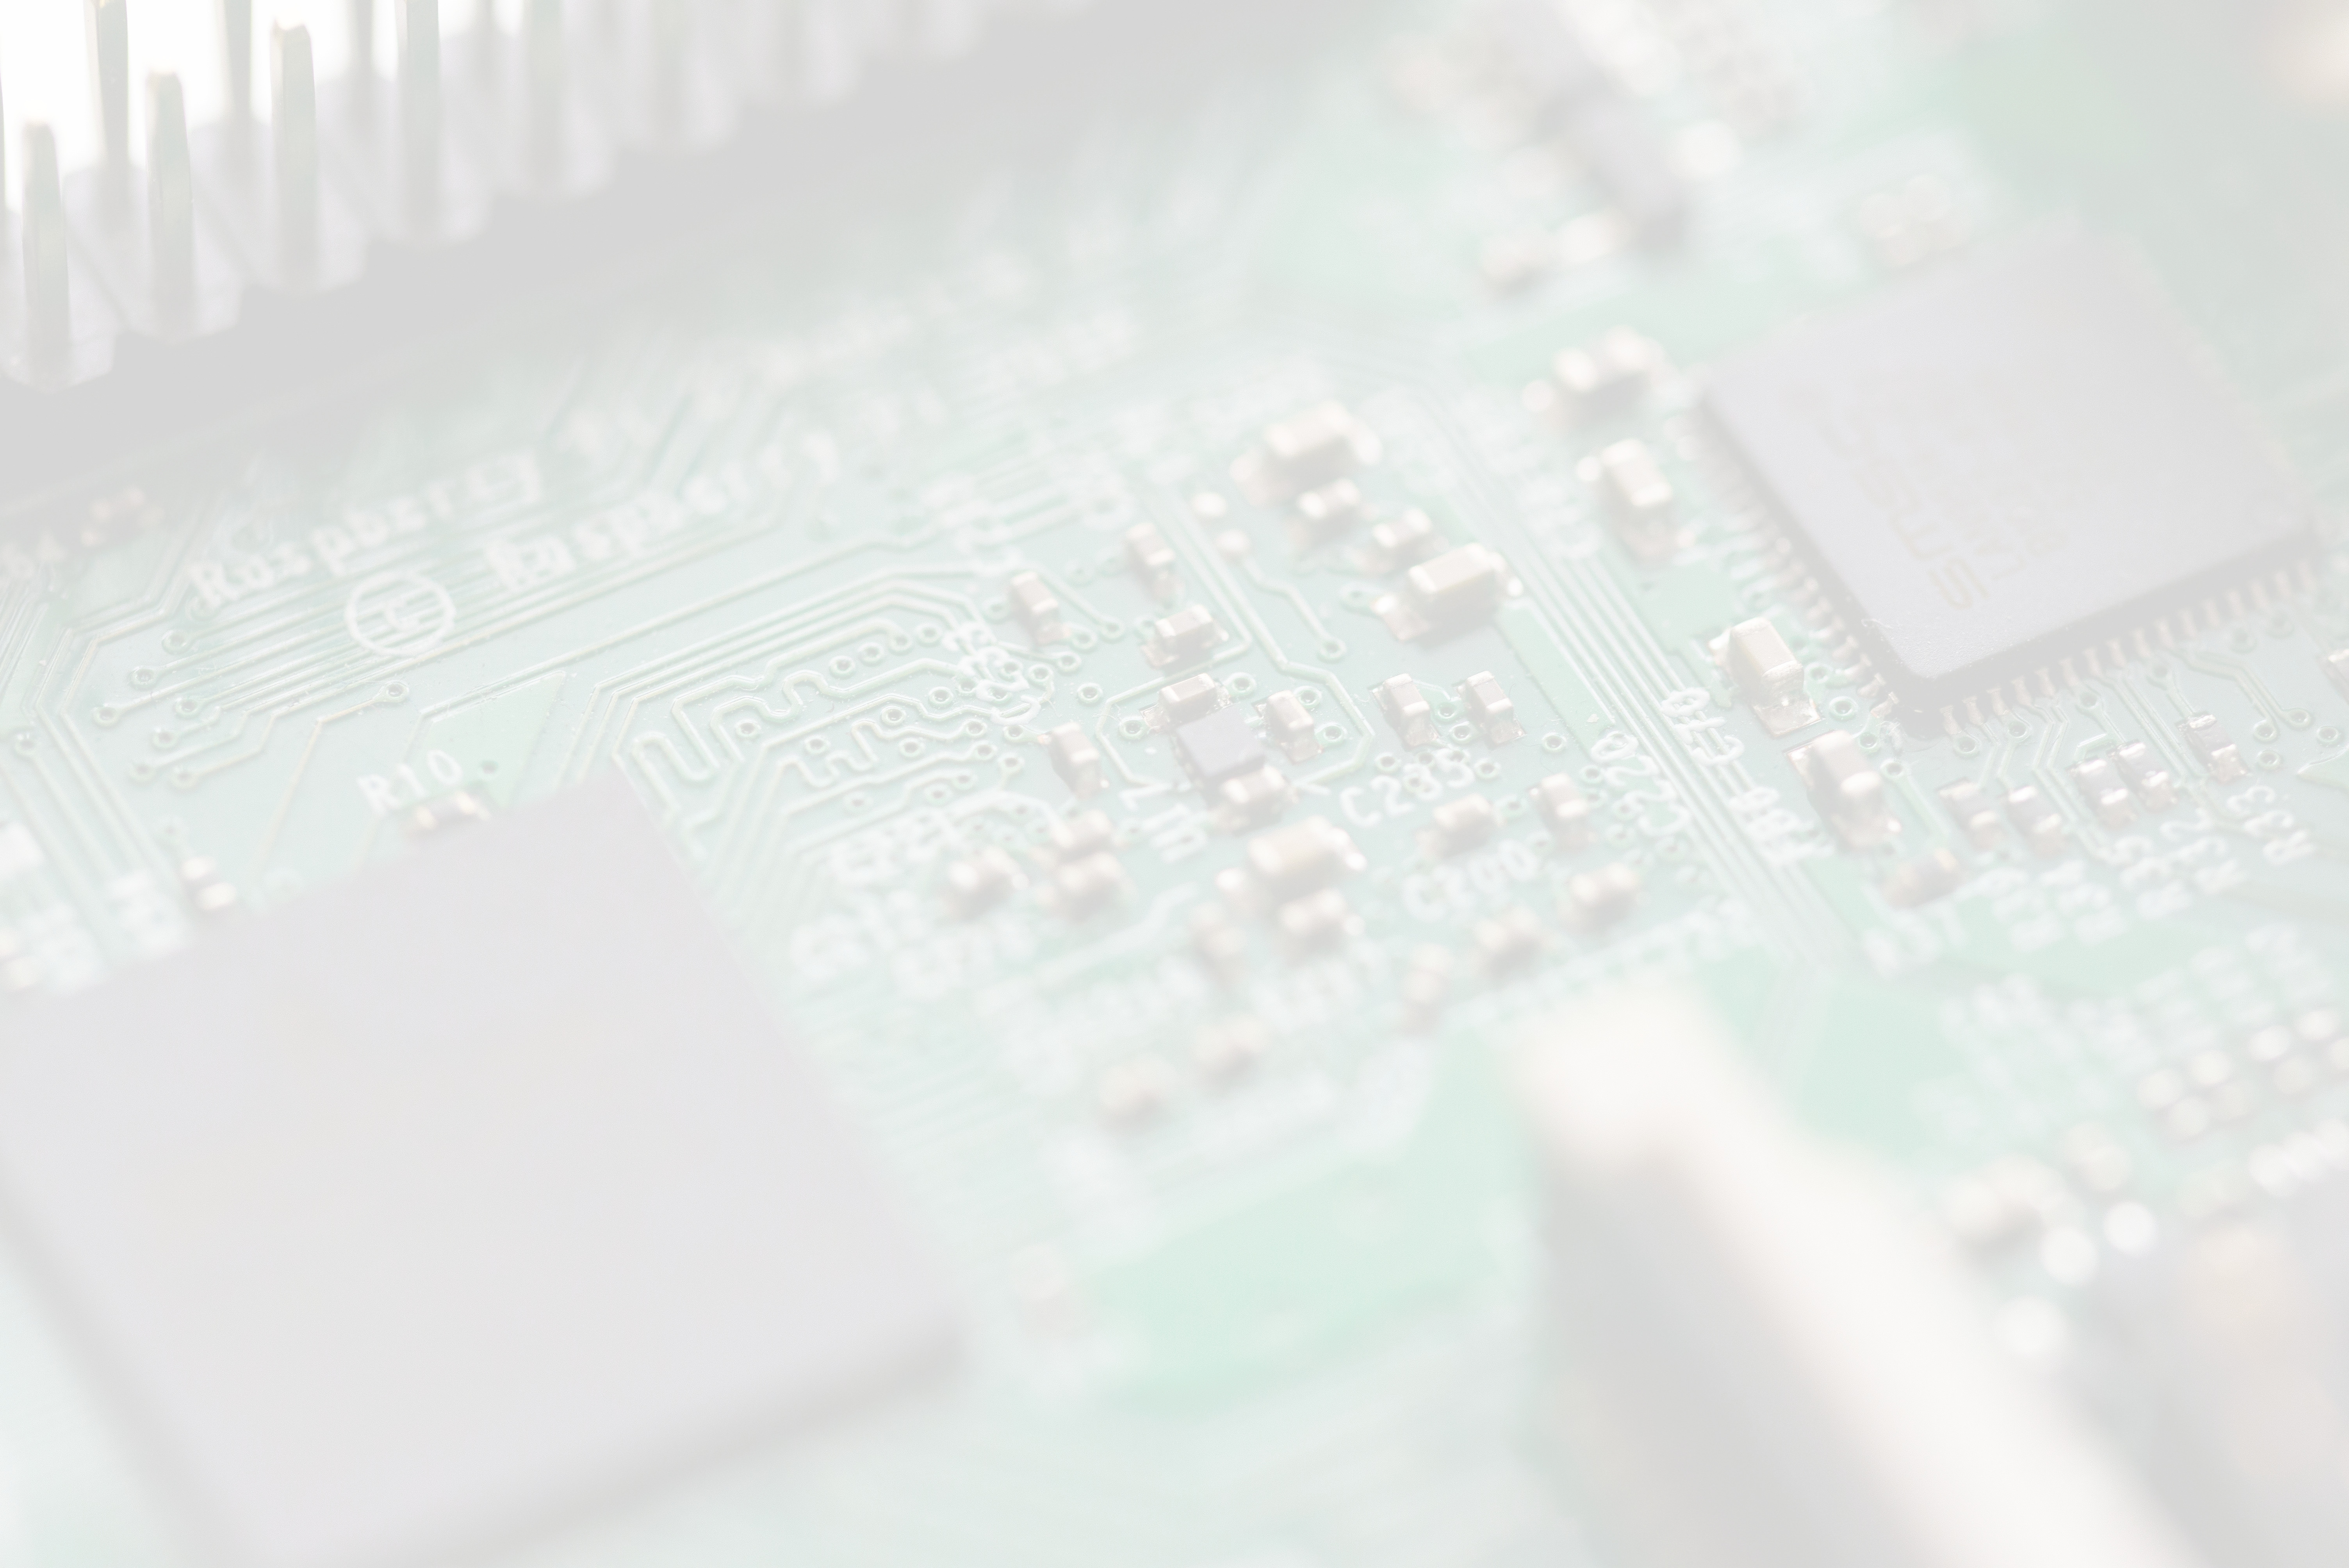
\includegraphics[height=\paperheight]{Images/Board.jpg}
        \vfill
    }}}

    \newcommand\leadbackgroundimage{
        \put(-5,0){
        \parbox[b][\paperheight]{\paperwidth+5px}{
        \vfill
        \centering
        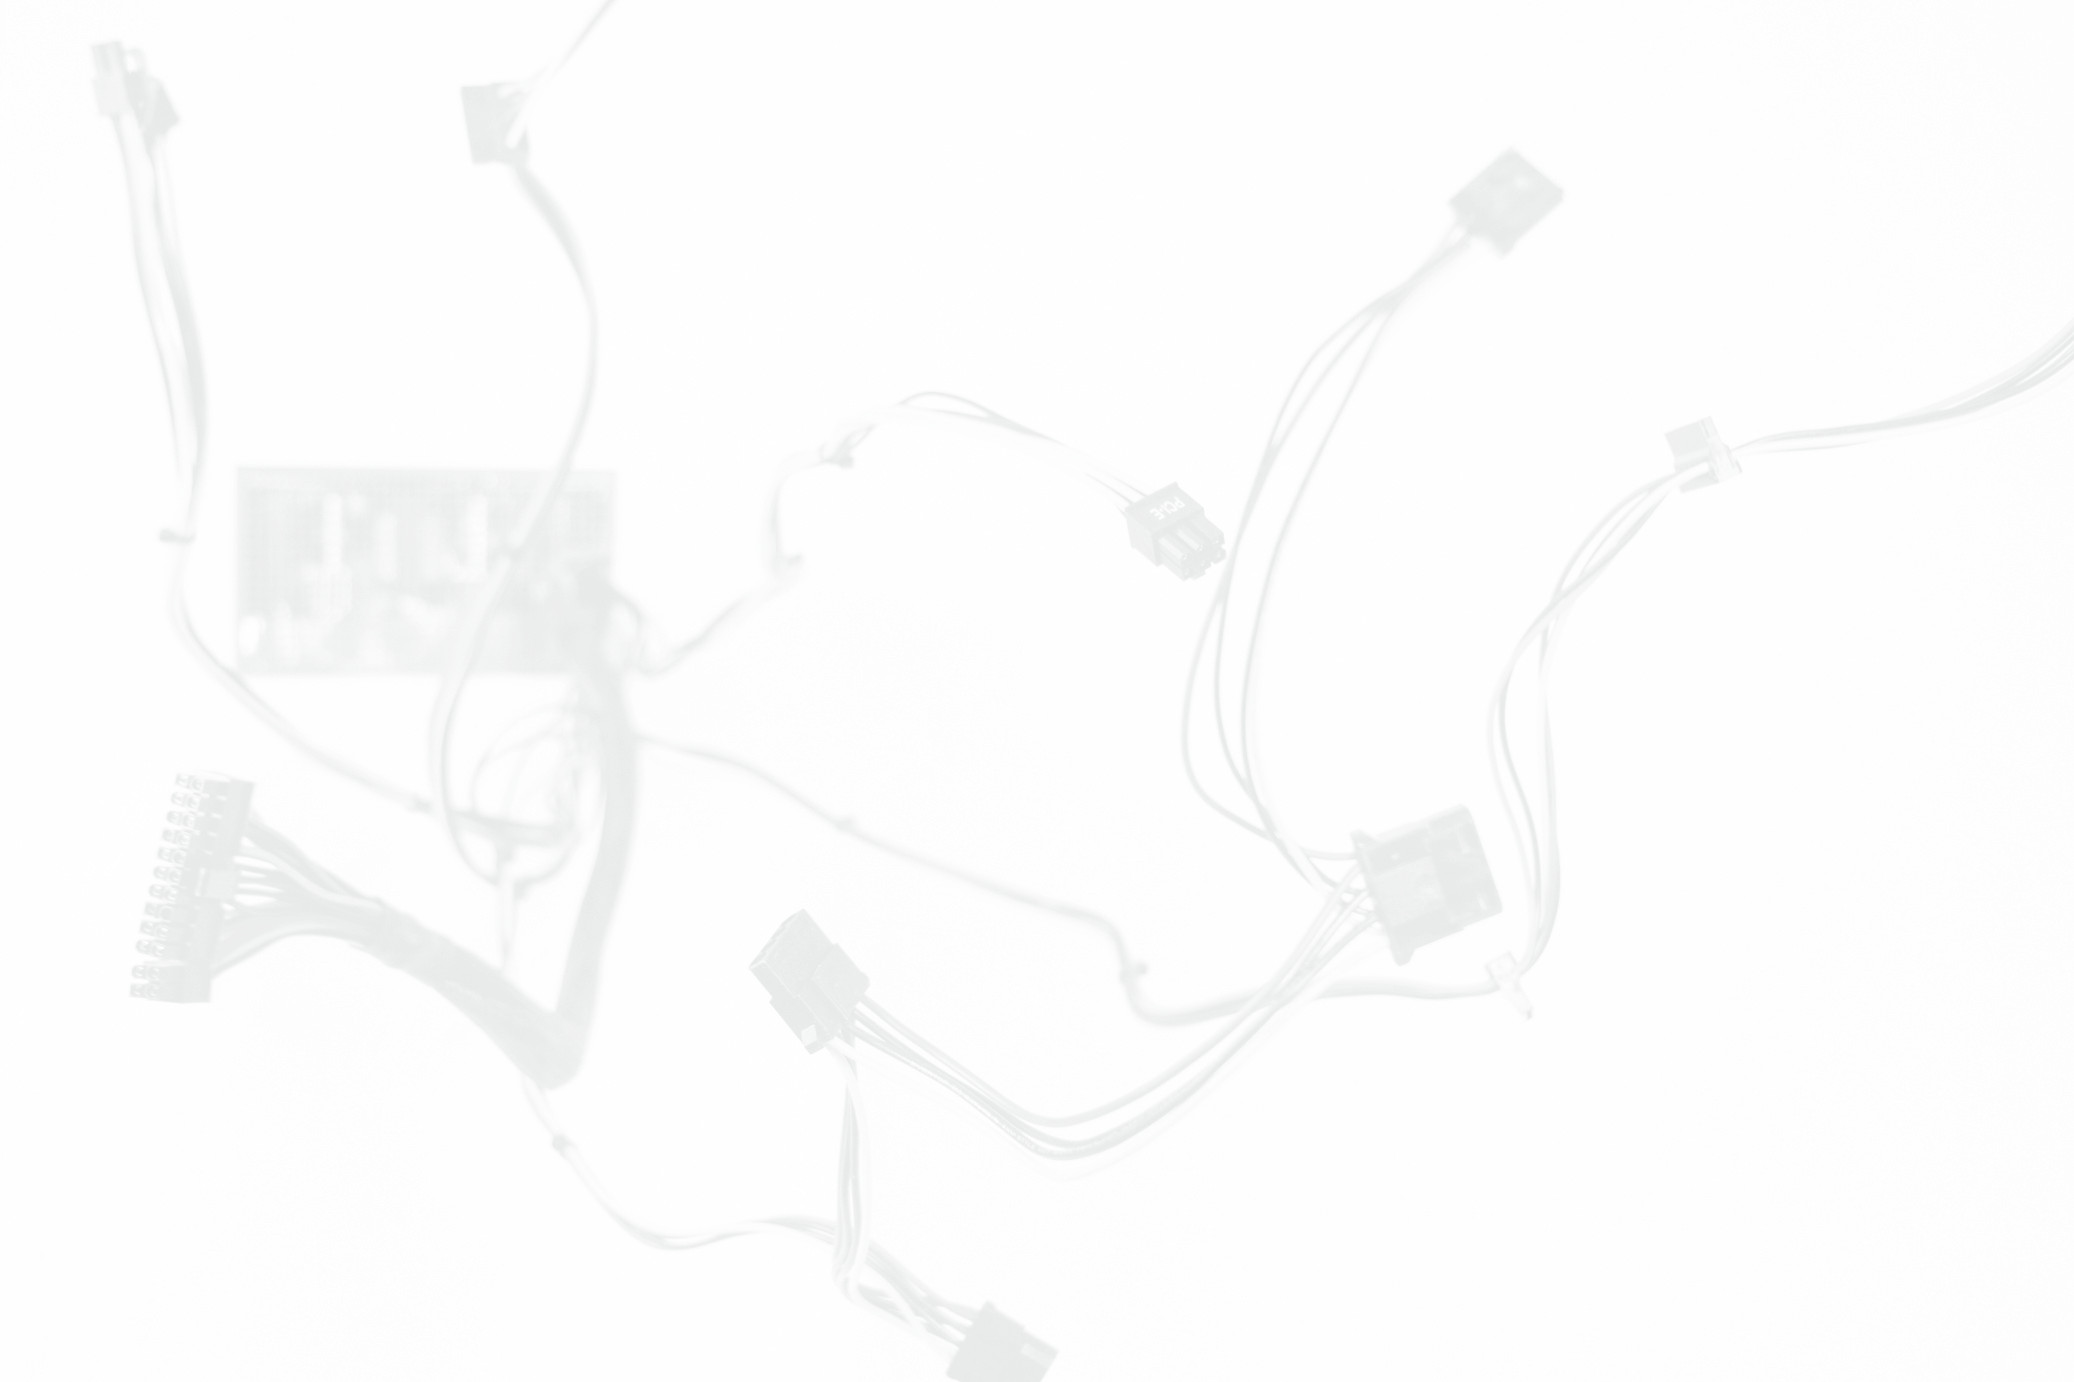
\includegraphics[height=\paperheight]{Images/Leads.jpg}
        \vfill
    }}}

    \newcommand\nesbackgroundimage{
        \put(-5,0){
        \parbox[b][\paperheight]{\paperwidth+5px}{
        \vfill
        \centering
        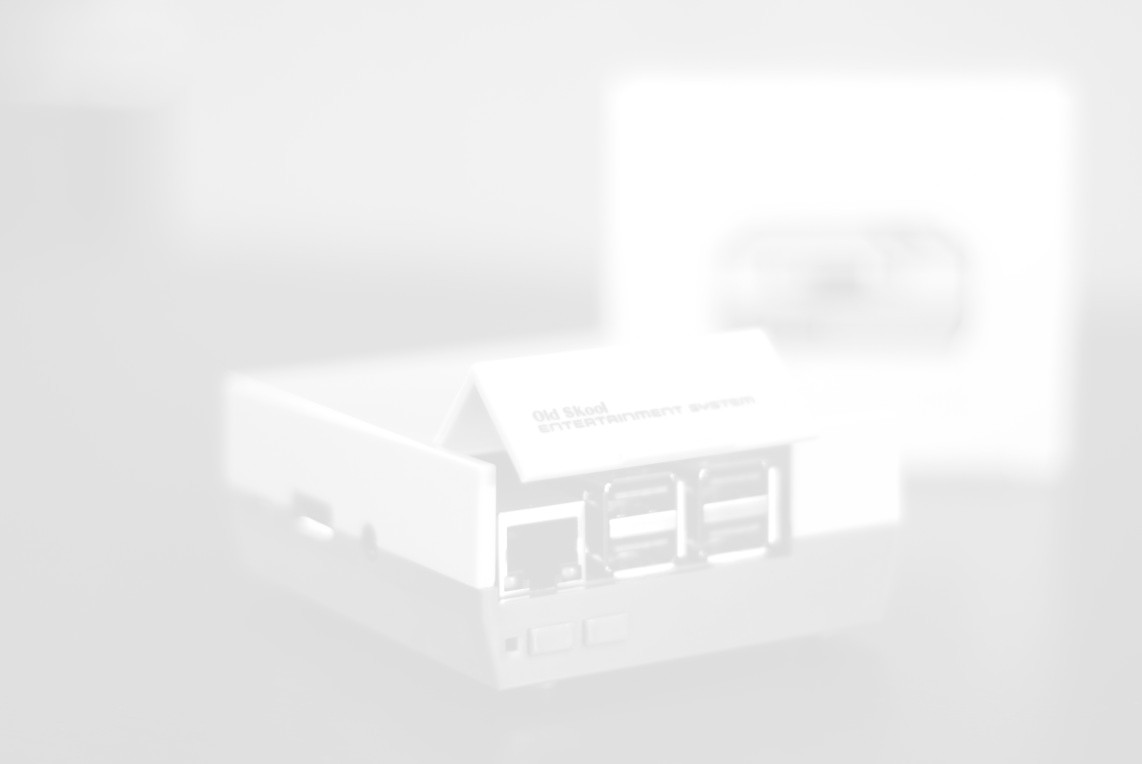
\includegraphics[height=\paperheight]{Images/NES.jpg}
        \vfill
    }}}

    \newcommand\makerbackgroundimage{
        \put(-5,0){
        \parbox[b][\paperheight]{\paperwidth}{
        \vfill
        \centering
        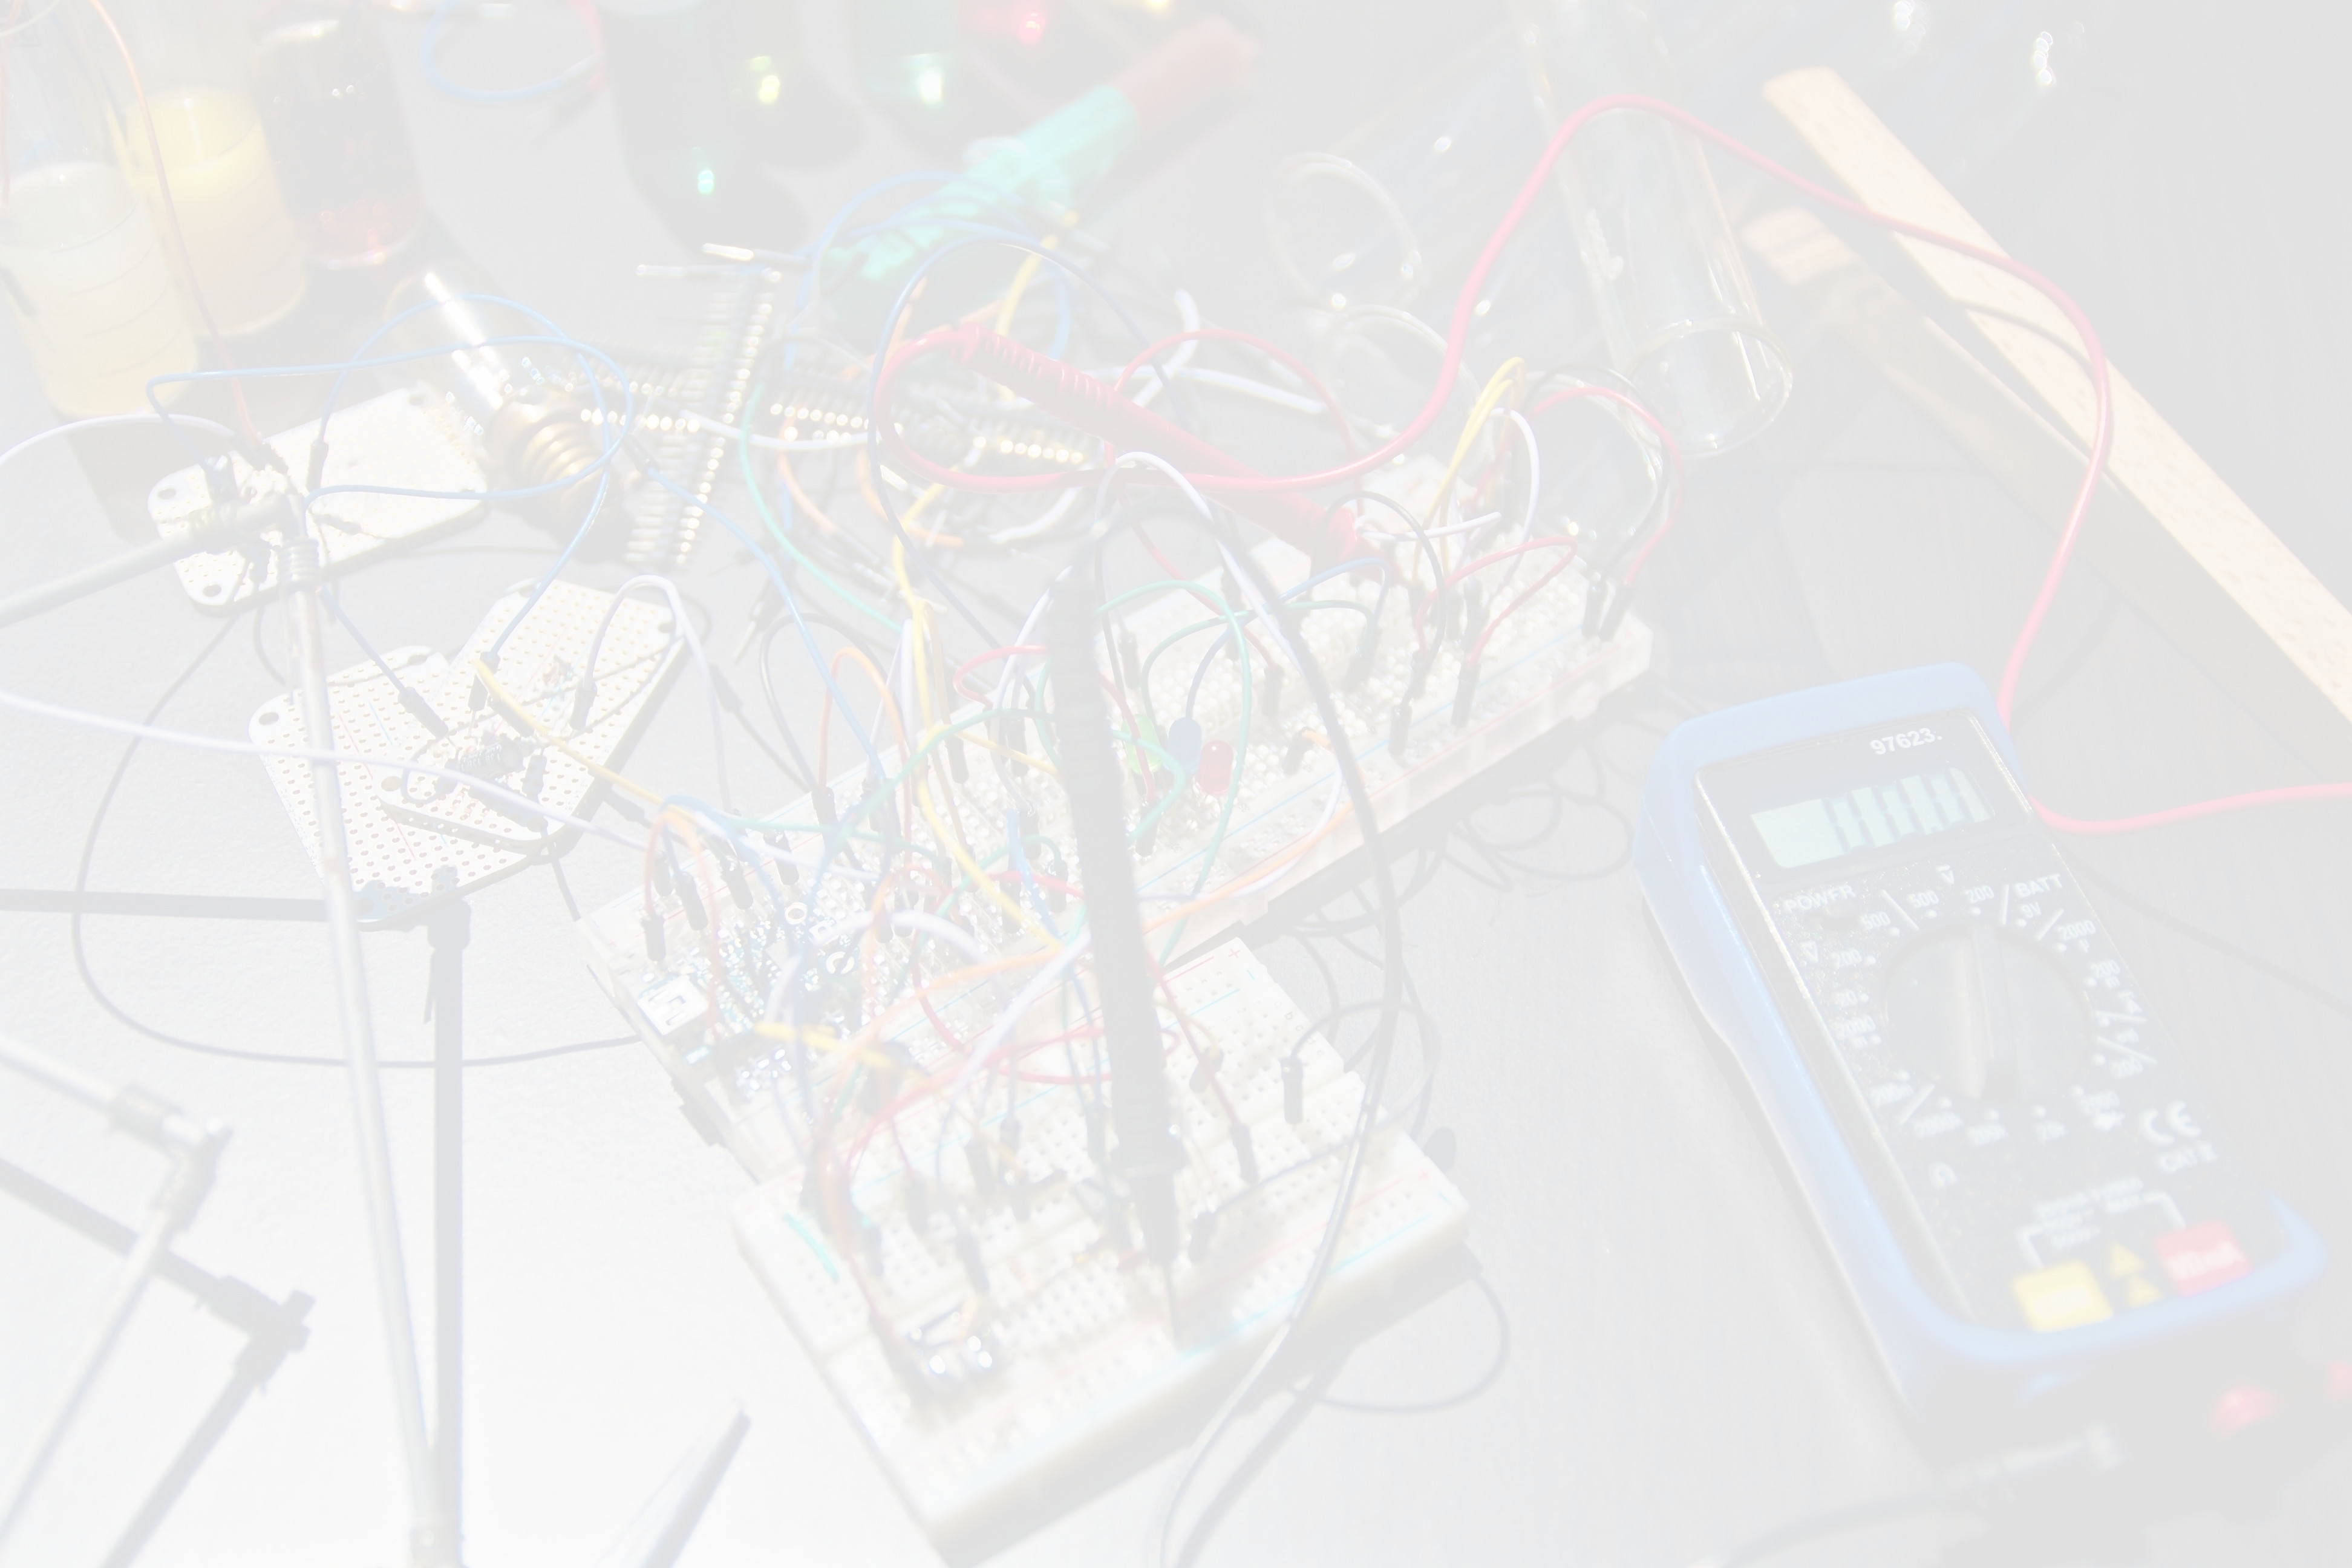
\includegraphics[height=\paperheight]{Images/Maker.jpg}
        \vfill
    }}}

    \newcommand\unobackgroundimage{
        \put(-5,0){
        \parbox[b][\paperheight]{\paperwidth}{
        \vfill
        \centering
        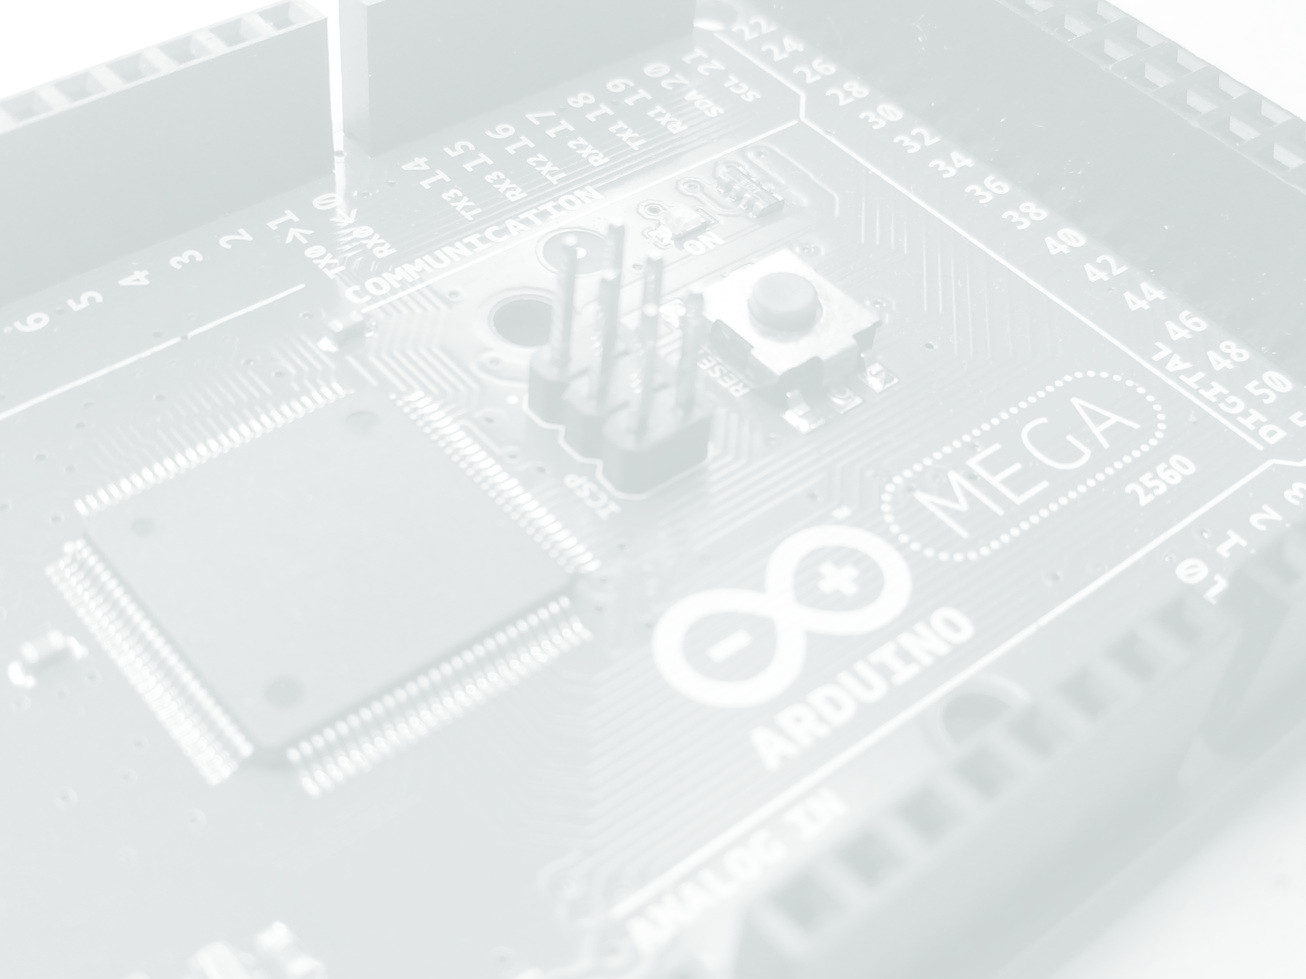
\includegraphics[height=\paperheight]{Images/Uno.jpg}
        \vfill
    }}}

    \graphicspath{ {Images/} }

    \title{\textbf{INFT3970 Major Project Scope Document \protect\\
    Distributed Monitoring System using Embedded Devices}}
    \author{
        Jay Rovacsek
        \texttt{c3146220@uon.edu.au}\\
        Dean Morton
        \texttt{c3252227@uon.edu.au}\\
        Josh Brown
        \texttt{c3283797@uon.edu.au}\\
        Jacob Litherland
        \texttt{c3263482@uon.edu.au}\\
        Lee Marron
        \texttt{c3263482@uon.edu.au}\\
        Edward Lonsdale
        \texttt{c3252144@uon.edu.au}
    }
    \date{\today}
    \hypersetup{
    colorlinks=true,
    linkcolor=black,
    filecolor=magenta,      
    urlcolor=blue,
    citecolor=red,
    linktoc=section,
    }
    \pagenumbering{arabic}

    \newlist{legal}{enumerate}{10}
    \setlist[legal]{label*=\arabic*.}

    \begin{document}

    \AddToShipoutPicture{\arduinobackgroundimage}

    \begin{titlingpage}
        \maketitle
    \end{titlingpage}

    \AddToShipoutPicture{\usbdocumentbackgroundimage}

    \tableofcontents
    
    \newpage

    \AddToShipoutPicture{\unobackgroundimage}

    \section{Executive Summary}
        \subsection{Background}
            Riding the wave of "IoT Revolution" \cite{Forbes}, this project will develop
            a low cost, easily deployable IoT product in any setting.
            \\
            IoT or \textit{The Internet of Things} has proven to be an explosive trend within
            the consumer electronics markets. Never before have such small versatile devices been
            available for general consumption, leading to an estimated combined business and
            consumer spending value in excess of \$6 \textit{trillion} dollars globally in 2018\cite{Forbes}.
            \par\noindent
            For the vast majority of consumers, both corporate and end-customer \cite{Mckinsey}, a large 
            movement toward both minimisation of waste and optimisation of spending is occuring
            on a global scale in the developed world, with the developing world rapidly following 
            this trend also\cite{SunNews}.
            \\
            Citing this movement, it would only be logical to create a simple to use set of devices 
            that allow for the monitoring and therefore optimisation of such measurables.
        \vspace{5mm}
        \subsection{Overview and Purpose}
            The concept of this project is to create a distributed system in which small 
            devices are used to monitor, log and analyse a number of select metrics from a 
            multitude of potential data points.
            \par\noindent
            The purpose of the project is to deliver a viable product that could be replicated
            for a reasonable price for both end-user and business alike. We believe the market to
            be on a precipice of further explosive growth, with the consumer market partially
            realised, but far from tapped by curent offerings.
            \par\noindent
            In this document we intend 
            \subsubsection{Metrics}
                The metrics measured included will be: 
                \begin{itemize}
                    \item Temperature
                    \item Humidity
                    \item Motion
                \end{itemize}
                We anticipate further development on the project to be viable post submission date,
                however realise the limitations of the current timeframe.
                \par
                Metrics measured would be viewable on a users dashboard, with data being able to be
                scoped to multiple filter requirements such as time, select edge cases or specific 
                locations.
                \\
                The end-goal being an ability for users to better determine inefficient or bad decisions
                they may make unwittingly in regards to home or business heating, coupled with the 
                impact of room utilisation.

    \newpage

    \section{Business Needs}
        As suggested in the executive summary and project background, the IoT market is expected 
        to rapidly grow in not only the current year but a number of future years to come. Accessibility and ease of use being major factors spurring the market into the current 
        state.
        \\
        This project aims to fill some of the gaps that exist within the expanding world of IoT
        by allowing end users irrespective of technological capability to easily partake in the 
        current market at a price position that doesn't reflect excessive or overly expensive 
        alternatives that exist.

        \subsection{Azure Hosting}
            Currently without extenuating circumstances against hosting within the cloud the
            decision to host in Azure applications seems to be the path of least resistance for
            the project in order to enable a globalised access to a single database to host 
            data.
            \\
            We recognise the flaws with hosting in the cloud also, such as data breach potential 
            (traditional methods or emerging threats\cite{SpectreAndMeltdown}), however also
            recognise with a limited span of time allowable for the project a more suitable 
            system design such as below is not suitable in the timeframe:
            \vspace{10mm}
            \begin{center}
                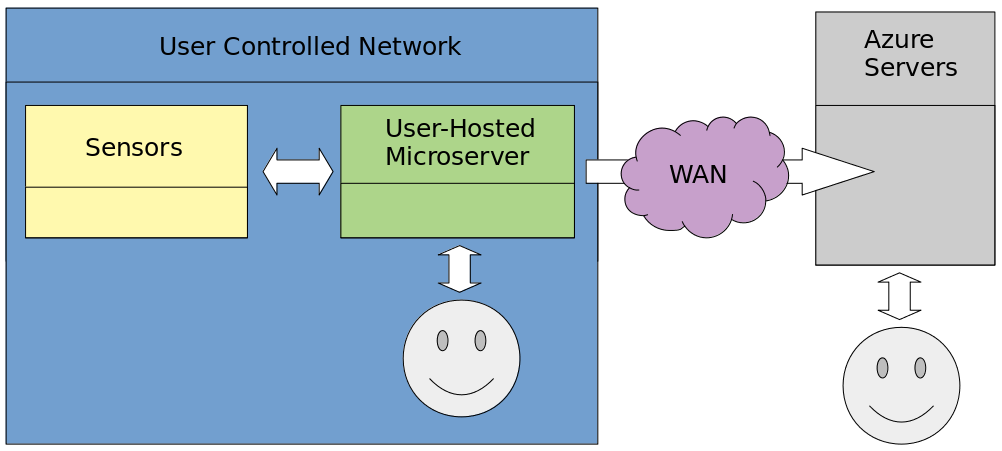
\includegraphics[width=350px]{Images/OptimalSystemDiagram.jpg}
            \end{center}
            Such a design would allow for users to maintain connectivity from their 
            own LAN:
            \begin{center}
                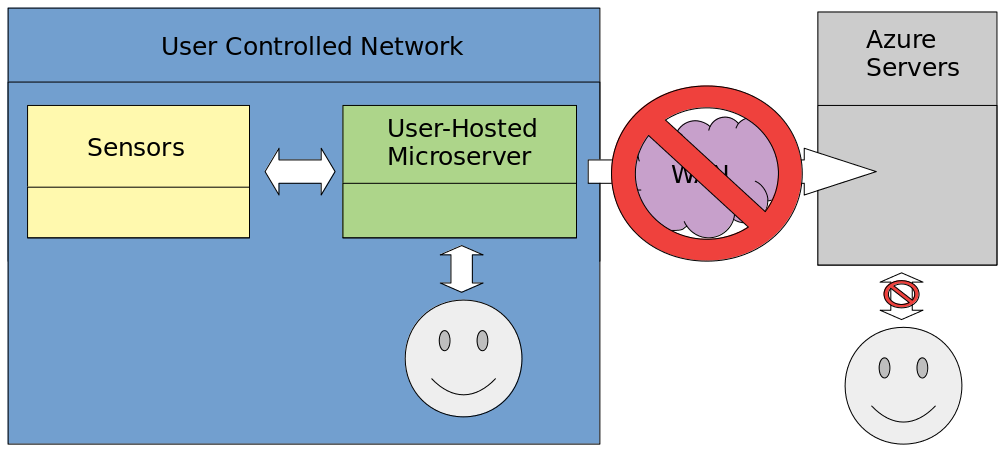
\includegraphics[width=350px]{Images/OptimalSystemDiagramAlternate.jpg}
            \end{center}

            \newpage

            Given time constraints we need to accept that the design of centralised 
            servers hosted within Azure achieves the same ability to serve the user information and maintain connectivity as required, but is more failable:

            \begin{center}
                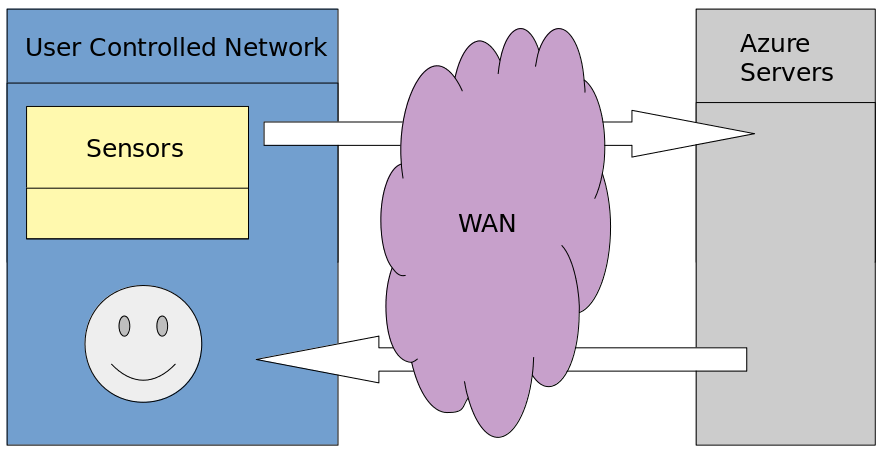
\includegraphics[width=350px]{Images/CurrentSystemDiagram.jpg}
            \end{center}
            In a network failure situation:
            \begin{center}
                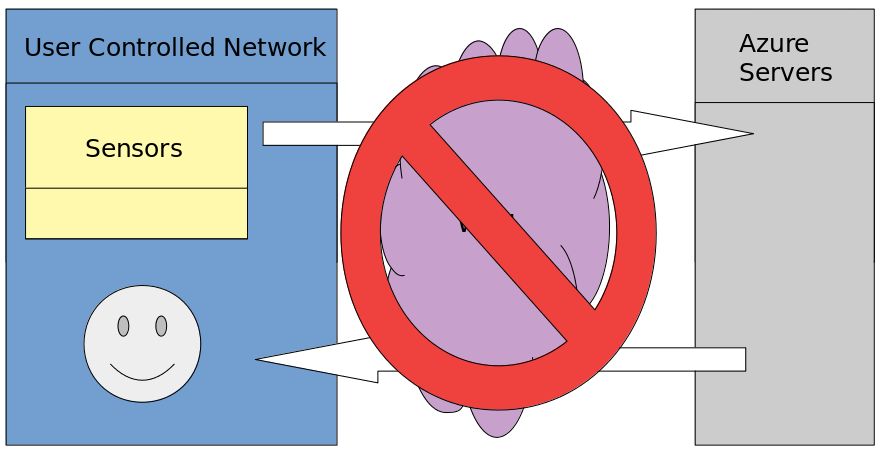
\includegraphics[width=350px]{Images/CurrentSystemDiagramAlternate.jpg}
            \end{center}

            Optimally the scope of the project would be expanded to development of
            the user hosted microservers that would act as middleware between
            the hosted servers and the sensors, this is a highly viable goal given
            technologies such as the RaspberryPi\cite{RPI} which under \$50AUD 
            can a number of Linux distributions or Windows IoT Core platform.
        
        \subsection{WLAN v Zigbee}
            Considerations to implement the network of devices was considered however given the requirement to purchase and implement a module
            to enable use of Zigbee, conventional WEP/WPA/WPA2 network options 
            were perfered. Both conventional WLAN networks and Zigbee would allow
            meshability between devices, requiring less of an impact on the user's
            network in a mixture of DHCP leases and wireless network congestion.

    \newpage
    \AddToShipoutPicture{\leadbackgroundimage}


    \section{Project Objectives}
        Within the timeframe still available to this project, we aim to develop and deploy a number of 
        IoT devices\cite{ESP8266} to a home enviroment or two and to track heat, humidity and motion of the
        dwelling to better understand the potential correlations of room use, heating and potential 
        inefficiencies created in areas such as 'High Traffic' spots (Loungerooms and Hallways)
        \\
        Optimally we ain to couple this with a mapping of the dwelling, allowing a more intuitive expression 
        of the data collected.
        \par
        We intend on using student subscriptions to leverage Azure for both website hosting and databasing 
        coupled with a small budget of roughly \$100-\$200 to purchase all required equipment which currently
        is expected to be:
        \begin{itemize}
            \item Arduino UNO3 Microcontroller\cite{UNO3}
            \item ESP8266 boards\cite{ESP8266}
            \item DHT11 Temperature and Humidity sensors\cite{DHT11}
            \item XC-4444 PIR Motion sensors\cite{XC-4444}
            \item Various required breadboards / generic electronics items
        \end{itemize}

        The overall goals of the project is to enhance our knowledge of of IOT sensor technology in the scope of exploratoring what this technology can achieve and expanding the paradigm of this technologies implementations. 
        \par
        Secondarily the group seeks to develop our ability to interface with middleware using a number of appropriate languages to create a frontend user interface for users to monitor/operate and perform data analytics on the system and a backend for data management system that interfaces with an SQL server implementation. 
        \par
        We intend in this project to showcase out abilities while expanding our capabilities and have an aim to deliver a prototype by week 9.

        \newpage
        \AddToShipoutPicture{\dronebackgroundimage}
        \section{Deliverables}
            The deliverables that are expected to be produced throughout the distributed monitoring system are broken into Four sections; Sensors, Database, UI and 
            analytics.
            \subsubsection{Sensors}
            \begin{itemize}
                \item Humidity Sensor can be created.
                \item Temperature Sensor can be created.
                \item Motion Sensor can be created.
                \item Sensors can be reprogrammed with different modules (Or have all modules avilable).
                \item Sensors ownership can be modified.
                \item Sensors cav connect to any 2.4gHz home network.
            \end{itemize}

            \subsection{Database}
            \begin{itemize}
                \item A new user account can be created.
                \item A new sensor can be registered.
                \item An admin can access user’s information (password hashed + salted)
                \item A user record can be edited.
                \item A sensor can be assigned to a user account.
                \item A sensor can be deleted from a user’s account.
                \item A sensor’s details can be edited.
                \item An admin can view raw data from all tables.
                \item An admin can edit data from tables.
                \item Password can be changed
                \item Email will be sent for resetting a forgotten password
                \item Email verification upon account creation
                \item Procedures and triggers for data analysis and querying 
            \end{itemize}
            
            \newpage

            \AddToShipoutPicture{\whitebackgroundimage}

            \subsection{User Interface}
            \begin{itemize}
                \item Login page for Users.
                \item Registration page for Users.
                \item Home page (Displaying an overview).
                \item Temperature page.
                \item Humidity page.
                \item Motion page.
                \item User able to access associated data.
                \item Graphs based on the user data.
                \item User able to customise graphs and Home page layout.
                \item Custom Analytic results.
                \item Email Suggestions section.
                \item Logout Page.
            \end{itemize}

            \subsection{Data Analytics}
            \begin{itemize}
                \item Administration able to view user data that has been depersonalised.
                \item Display Recommendations and habits to the User.
                \item Showing different trends around a user’s house using the different modules.
            \end{itemize}
            \noindent
            Having a Data Analytics major within our group we expect the data collected may contain interesting information. \\
            An analytic module will be used to parse data for each user and display recommendations and habits from the data.
            
            \subsubsection{Temperature Module}
                The analytic module will be able to tell the users how different the temperature is around their house and see trends on room temperatures. This will also be able to be used to give recommendations on what rooms need heating/cooling and what rooms do not benefit from heating or cooling.
            \subsubsection{Humidity Module}
                The analytic module will be able search through the data and view what rooms and areas of the house are the most humid. This allows the user to keep an eye on the moisture that is in their homes like a wardrobe or kitchen pantry. Another use for the humidity module is alongside the temperature module to give suggestions to the user if they should turn on/off Air-conditioning units.
            \subsubsection{Motion Module}
                The analytic module will be able to see trends and habits on behaviour as they move through their home. By using this information the user will be able to see what rooms are high traffic areas and at what times of the day this high concentration of movement occurs. Through this it can also be used to tell when outliers occur for security purposes. Such as late night movement in a shed could be an intruder and the user will be notified with this uncommon event.

            \newpage

        \subsection{Milestones}
        A number of highly important milestones have been already scheduled as below;

        \begin{center}
            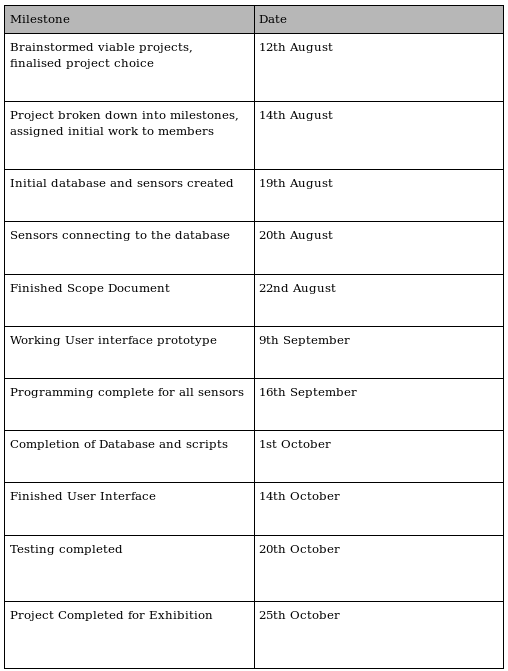
\includegraphics[width=300px]{Images/Milestones.jpg}
        \end{center}

        \newpage

            Otherwise milestones for the project include are split into a number of 
            concurrently developed sub-sections:
            \\
            \begin{legal}
                \item Database:
                \begin{legal}
                    \item Database Pilot (Including creation and design)
                    \item Review and Testing of Database
                    \item Optimisation of datatypes used in each table
                    \item Implementation of indexing and other optimisations to avoid big O issues.
                    \item Final database implementation.
                \end{legal}
                \item Backend:
                \begin{legal}
                    \item Decision of framework to be used
                    \item Initial POC on framework
                    \item Feature implementations: 
                    \begin{legal}
                        \item Implementation of PING GET endpoint to avoid sending of data unnecessarily
                        \item Implementation and testing of POST endpoints:
                        \begin{legal}
                            \item Temperature
                            \item Humidity
                            \item Motion
                        \end{legal}
                        \item Implementation and testing of application helpers to aid front-end data sourcing
                    \end{legal}
                    \item Refactor existing code
                    \begin{legal}
                        \item Peer review of code, implementation of required changes
                    \end{legal}
                \end{legal}
                \item Front End:
                \begin{legal}
                    \item Initial implementation of POC dashboard
                    \item Initial POC of authentication using a login page
                    \item Review of code by peers
                    \item Migrate dashboard behind successful login page
                    \item Improvements and refactoring of dashboarding code
                    \item Review and refactor to suit all devices commonly used to browse websites.
                    \item Implement required bootstrap/css framework to handle display of data.
                    \item Final peer review and refactor
                \end{legal}
                \newpage
                \item Sensors:
                \begin{legal}
                    \item Pilot testing of potential boards (UNO3\cite{UNO3} / ESP\cite{ESP8266} / RPI\cite{RPI} / OPI\cite{OPI})
                    \begin{legal}
                        \item Code feasability report on each board, considerations on support from community 
                        and team ability
                        \item Review of boards and decision on main boards to use
                    \end{legal}
                    \item Implement monitoring for chosen metrics:
                    \begin{legal}
                        \item Temperature
                        \item Humidity
                        \item Motion
                    \end{legal}
                    \item Implement networking on boards
                    \begin{legal}
                        \item Determine viability of WPA2-Enterprise connectivity
                    \end{legal}
                    \item Implement json generation on boards
                    \item Implement PING request functionality to check web server is up or not
                    \item Test API communication
                    \item Design and print 3D case for boards
                    \item Deploy boards to various locations
                \end{legal}
                \item Documentation
                \begin{legal}
                    \item Generate POC documentation from project
                    \item Generate scope document
                    \item Comment code extensively for readability
                    \item Document APIs
                    \item Document database design, with considerations of optimisation and required modifications
                    \item Generate user guide for final product
                    \item Generate final report
                \end{legal}
            \end{legal}

        \newpage
        \AddToShipoutPicture{\makerbackgroundimage}

    \section{Key Roles in Project}
        Key roles defined for the project include the below:
        \vspace{10mm}
        \begin{center}
            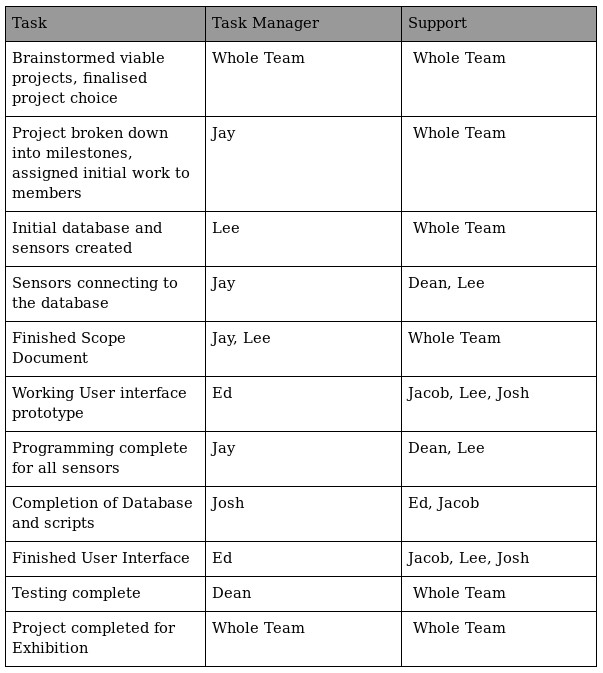
\includegraphics[width=\textwidth]{Images/KeyRoles.jpg}
        \end{center}
    \newpage

    \AddToShipoutPicture{\boardbackgroundimage}

    
    \section{Technical Requirements}
        \subsection{Generalised Requirements}
            The team collaboratively have agreed on a few generalised requirements of the project
            including:
            \begin{itemize}
                \item Ease of use: The devices must be able to used by a nontechnical user, they must
                be supplied in such a way that an ability to place the device in place, and connect power
                are the largest difficulties that the end user encounters.
                \item Abstraction of underlying technologies: as a byproduct of the requirement of ease-of-use
                the devices and web application should not require the end user to have any knowledge of the 
                underlying technolgies used.
            \end{itemize}
        \subsection{Data Requirements}
            Requirements for raw data be stored in an online database are only access
            for the development resources to be able to access any suitable cloud account, 
            self-host on a local machine or debug required functions in the application with 
            localised data generation via ajax queries of similar methods.
            
            \subsubsection{Azure}
                Azure is a likely candidate for the Database and website hosting, The database will be used to store 
                all the data that is sent from the sensors. The uptime of the database the web application is vital 
                to the user experience and the success of the project. Azure provides this security 
                with 99.95\% uptime \cite{AzureUptime}.

        \subsection{Hosting Enviroment}
            Pages for the site itself will require a suitable host either cloud or local which
            supports .NETcore 2.0\cite{DotNetCore2} and suitable network access to reach a
            required TSQL\cite{TSQL} database hosted by the team.
        
        \subsection{Network Connectivity}
            Functioning network connectivity will be heavily depended on by the project,
            all of the sensors will be connected to a local network wirelessly which will enable the boards
            to post data at the API endpoint at either \url{https://www.inft3970.com} (Parked domain) or 
            \url{https://inft3970.azurewebsites.net} (Currently functioning endpoint)
            \par
            Requirements for the user to maintain a 2.4gHz enviroment will exist, as without this an expansion board
            or alternate boards will be required isntead of the proposed ESP8266\cite{ESP8266} and UNO3\cite{UNO3}.
        
        \subsection{User Requirements}
            The users of the system will need to be confident in browsing webpages and accessing them. Generally
            we recognise any device with browser functionality will suit the purpose, and development will use a 
            mixture of Firefox\cite{Firefox} or Chromium\cite{Chromium} based browsers to find all possible bugs 
            within the project span.
            \\
            The lack of an adblocker or similar addons for the chosen browsing enviroment would be suggested also,
            third party javascript libraries are likely to be used and cannot be assured to function under such 
            enviroments including modification or blocking of traffic/assets.
        
        \newpage

        \subsection{Development Requirements\cite{DevelopmentResources}}
            A number of softwares will be required by the development team in order to complete the project,
            these softwares may include:
            \begin{itemize}
                \item SQL management studio to manage the database. Azure is using TSQL which can be managed by SQL management studio 
                on the developers local machine.
                \item Visual studio to develop the front and back-ends of the web application. 
                \item Visual Studio Code to develop elements of the front-end
                \item Arduino IDE software for editing/flashing the boards in C/C++.
            \end{itemize}

        \newpage

    \section{Limitations}
        It is important to acknowledge the limitations of this project, given that this project is taking place 
        in a compressed format it will primarily be an exploratory exercise in IOT sensor technology and its 
        ability to interface with middleware, frontend/backend and an SQL server implementation.
        \vspace{10mm}
        In order to managing expectations we are primary focused on heat,humidity and motion, this proof of 
        concept implementation reduces the risk of under delivering on expectations.
        
        \subsection{Device Limitations}
            The ESP8266 is limited to the 2.4gHz wireless spectrum, and therefore a number of modern wireless
            networks may prove incompatible with the device. This is only a small hinderence to the device as
            most modern networks will use both 2.4 and 5.1gHz spectrums. Furthermore the 2.4gHz spectrum is 
            better suited to longer distance connections than the 5.1gHz range, and even in the most
            heavily congested of wireless areas it would be reasonable to expect the payload from the ESP would
            have no issues at a measly 200bytes on average.
            
            \subsubsection{Security Concerns}
            Issues related to security on the publicly open API endpoints hosted in Azure prove to be hindered
            by the limitations of the devices. We are currently investigating potential fixes for the current
            implementation in which requests over https connections should ensure a level of security over 
            current use of plain http.
            \\
            Implementation of a method that would allow access to a preflashed public key to be used for encryption
            purposes of sensitive json data before it even leaves the device would be an excellent addition to 
            the project, however both scope and inefficiencies of pub/private key encryption are reasons against
            this idea.
        
        \subsection{Development Limitations}
            Limitations of development experience may exist within the group with only 2 software engineering majors
            present. We expect that these members will be able to assist the other members in potential problem 
            areas and expect the use of code versioning will alleviate any potential miscommunications in code 
            modification and submission.
            \\
            Factors potentially negating this issue include a base level of programming knowledge being shared across
            all members of the team, with a heavy level of experience in C\# programming.

            \subsubsection{Framework Limitations}
                We may experience some level of difficulties with the chosen framework of .NETCore 2.0 in development
                as only a limited number of the team have experienced .NETCore MVC application programming or 
                .NETCore API programming. 
                \\
                We expect however the time required for upskilling and learning the framework will provide a positive
                time return if not purely allowing team members a new skill in which to take to potential employment 
                opportunities into the future.
        
        \newpage

    \begin{thebibliography}{9}
        \raggedright
        \bibitem{Forbes}
            Forbes article: Top 8 IoT trends of 2018:
            \url{https://www.forbes.com/sites/danielnewman/2017/12/19/the-top-8-iot-trends-for-2018/}
        \bibitem{Mckinsey}
            Mckinsey article: Value of digitizing the physical world:
            \url{https://www.mckinsey.com/business-functions/digital-mckinsey/our-insights/the-internet-of-things-the-value-of-digitizing-the-physical-world}
        \bibitem{SunNews}
            Sun News article: China; Largest Renewables Producer:
            \url{http://sunnewsonline.com/china-is-worlds-largest-renewable-energy-producer-consumer/}
        \bibitem{ESP8266}
            ESP8266 Information Page:
            \url{http://esp8266.net/}
        \bibitem{XC-4444}
            Jaycar XC-4444 Datasheet:
            \url{https://www.jaycar.com.au/medias/sys_master/images/9105858396190/XC4444-dataSheetMain.pdf}
        \bibitem{DHT11}
            Jaycar Resources; DHT11 Datasheet:
            \url{https://www.jaycar.com.au/medias/sys_master/images/9091897786398/XC4520-dataSheetMain.zip}
        \bibitem{DotNetCore2}
            .NETCore SDK Download Page:
            \url{https://www.microsoft.com/net/download}
        \bibitem{TSQL}
            TSQL Server Download Page:
            \url{https://docs.microsoft.com/en-us/sql/t-sql/language-reference?view=sql-server-2017}
        \bibitem{AzureUptime}
            Azure Uptime SLA:
            \url{https://azure.microsoft.com/en-au/support/legal/sla/app-service/v1_4/}
        \bibitem{UNO3}
            Arduino UNO3 Store Page:
            \url{https://store.arduino.cc/usa/arduino-uno-rev3/}
        \bibitem{Firefox}
            Firefox:
            \url{https://www.mozilla.org/en-US/firefox/}
        \bibitem{Chromium}
            Chromium:
            \url{https://www.chromium.org/}
        \bibitem{RPI}
            RaspberryPi Organisation Page:
            \url{https://www.raspberrypi.org/}
        \bibitem{OPI}
            OrangePi Website:
            \url{http://www.orangepi.org/}
        \bibitem{SpectreAndMeltdown}
            Spectre and Meltdown explaination page:
            \url{https://meltdownattack.com/}
        \bibitem{Unsplash}
            Unsplash Website:
            \url{https://unsplash.com}
        \bibitem{DevelopmentResources}
            Development resources:
            \begin{center}
                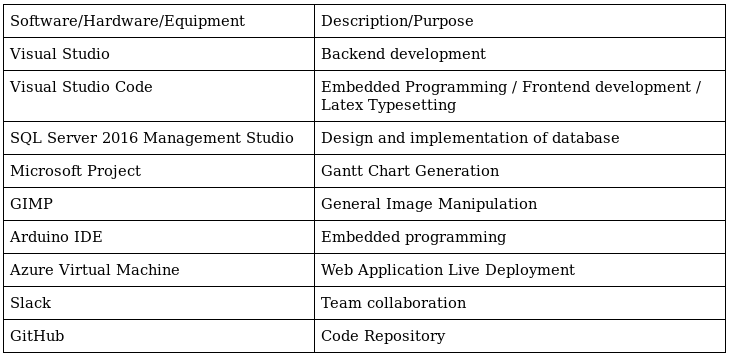
\includegraphics[width=400px]{Images/DevelopmentResources.jpg}
            \end{center}
    \end{thebibliography}

    All image backgrounds are images from Unsplash, a provider of free and openly
    licensed images\cite{Unsplash}

    \end{document}
